\documentclass{standalone}

\usepackage[english]{babel}
\usepackage[utf8]{inputenc}
\usepackage[T1]{fontenc}

\usepackage{amsmath, amssymb}

\usepackage{tikz}

\begin{document}

    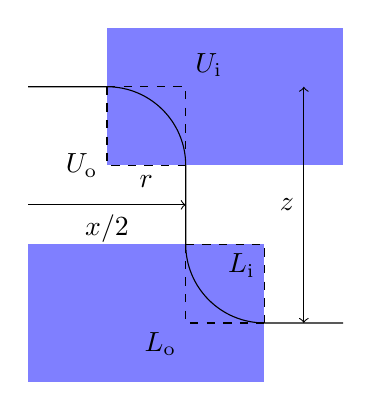
\begin{tikzpicture}
        \pgfmathsetmacro{\sizeX}{4}
        \pgfmathsetmacro{\sizeZ}{3}
        \pgfmathsetmacro{\cornerRadius}{1}
        \pgfmathsetmacro{\rectangleX}{3}
        \pgfmathsetmacro{\rectangleZ}{1.75}

        \fill[color=blue, opacity=0.5] (\sizeX/2-\cornerRadius, \sizeZ-\cornerRadius)
            rectangle ++(\rectangleX, \rectangleZ);
        \fill[color=blue, opacity=0.5] (\sizeX/2+\cornerRadius, \cornerRadius)
            rectangle ++(-\rectangleX, -\rectangleZ);

        \draw (0, \sizeZ) -- (\sizeX/2-\cornerRadius, \sizeZ)
            arc [start angle=90, end angle=0, radius=\cornerRadius]
            -- (\sizeX/2, \cornerRadius)
            arc [start angle=-180, end angle=-90, radius=\cornerRadius]
            --++ (\sizeX/2-\cornerRadius, 0);

        \draw[dashed] (\sizeX/2-\cornerRadius, \sizeZ) --++ (0, -\cornerRadius)
            node[left] {$U_\text{o}$}
            -- node[below] {$r$} ++ (\cornerRadius, 0);
        \draw[dashed] (\sizeX/2-\cornerRadius, \sizeZ) --++ (\cornerRadius, 0)
            node[above right] {$U_\text{i}$}
            --++ (0, -\cornerRadius);
        \draw[dashed] (\sizeX/2, \cornerRadius) --++ (0, -\cornerRadius)
            node[below left] {$L_\text{o}$}
            --++ (\cornerRadius, 0);
        \draw[dashed] (\sizeX/2, \cornerRadius) --++ (\cornerRadius, 0)
            node[below left] {$L_\text{i}$}
            --++ (0, -\cornerRadius);

        \draw [->] (0, \sizeZ/2) -- node[below]{$x/2$} ++ (\sizeX/2, 0);
        \draw [<->] (\sizeX/2 + \cornerRadius + \sizeX/8, 0) -- node[left] {$z$} ++ (0, \sizeZ);
    \end{tikzpicture}

\end{document}
